\begin{figure}[ht!]
\centering
	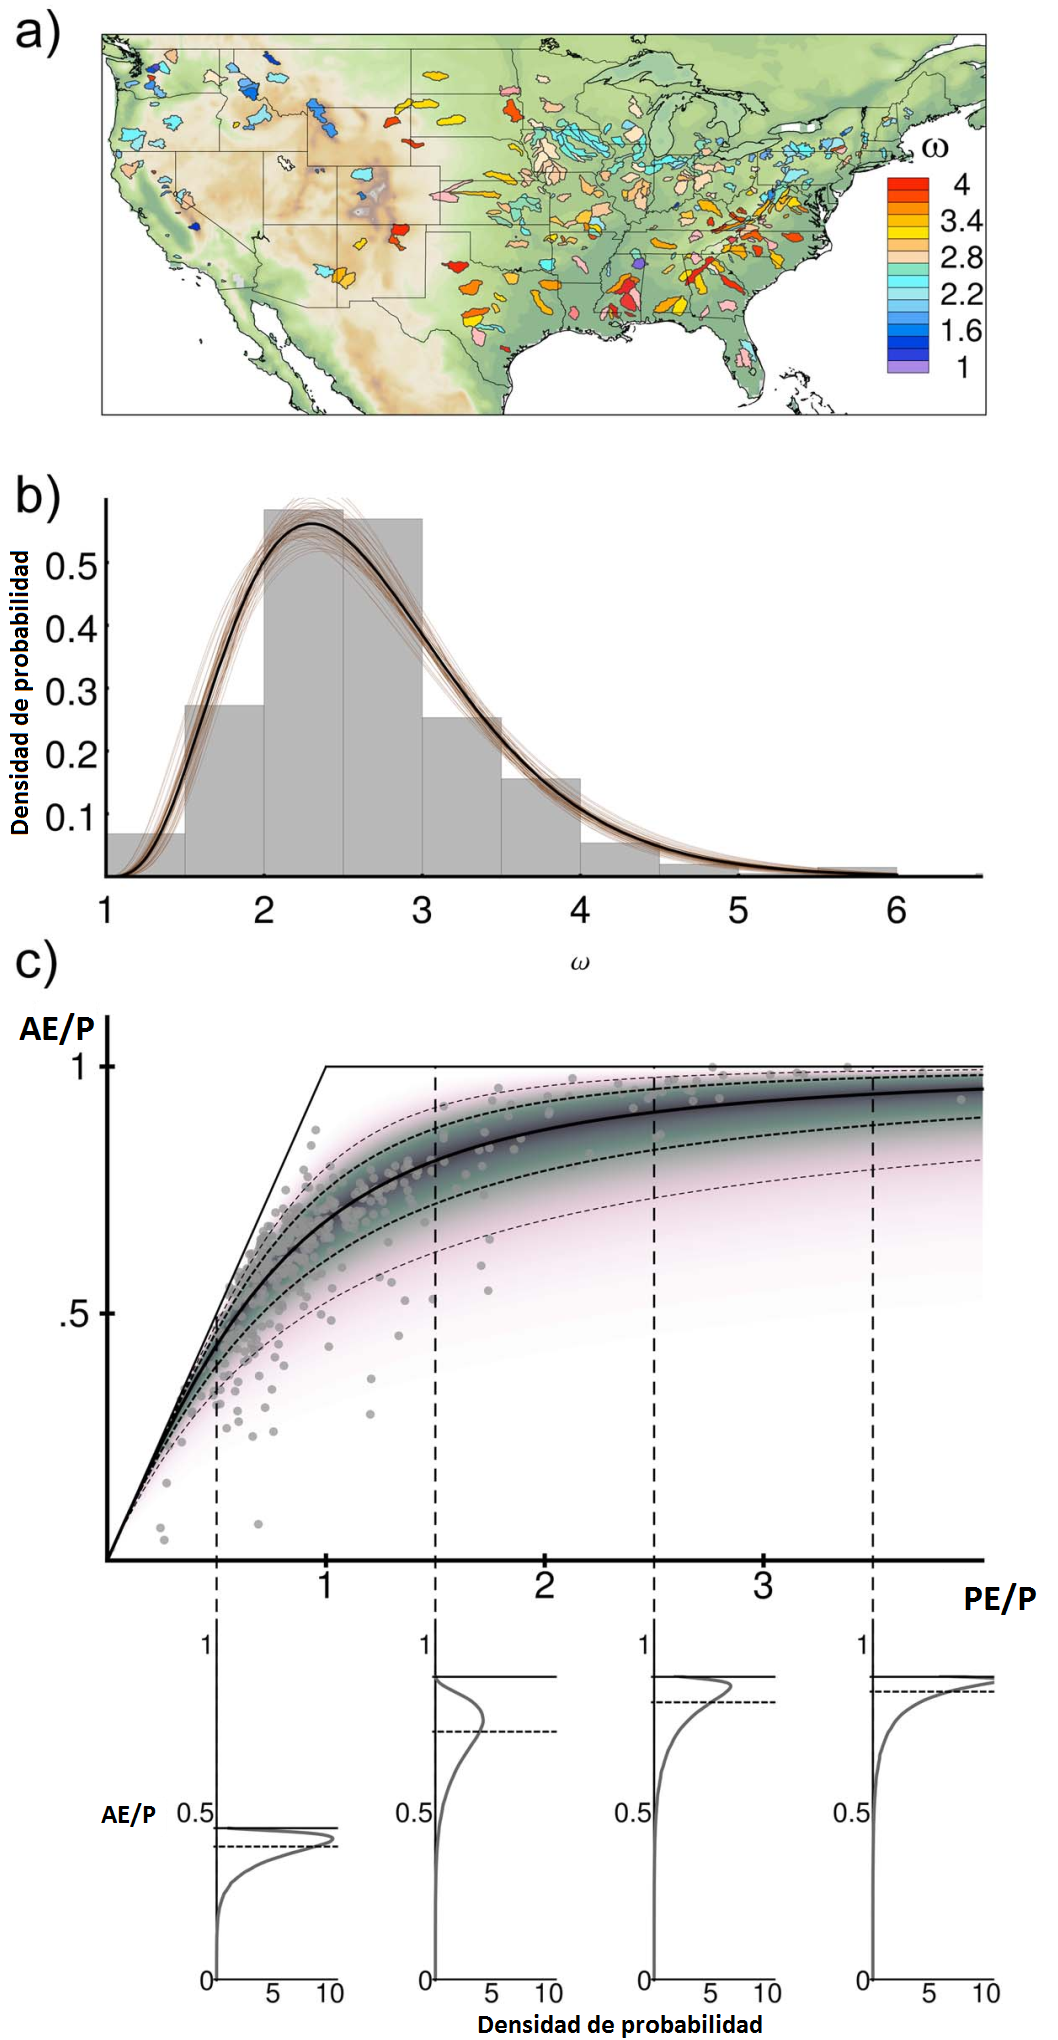
\includegraphics[scale=0.33]{Images/Greve03.png}
	\caption{a) Conjunto de 411 cuencas del MOPEX con su respectivo valor $\omega$. b) Histograma de todos los valores $\omega$ (barra gris) en conjunto con la distribución gamma ajustada (linea negra) y una muestra (bootstrapped) de distribuciones (lineas marrones). c) El enfoque de Budyko probabilístico estimado para las 411 cuencas del MOPEX. La distribución gamma es ajustada y utilizada para calcular la distribución de Budyko y las distribuciones de probabilidad condicionales para $PE/P = 0.5, 1.5, 2.5, 3.5$ (abajo). Las cuencas se muestran como puntos en gris.}
	Fuente: \citet{Greve2015}.
	\label{fig:Greve03}
\end{figure}